\section{Introduction} \label{sec:introduction}
Il task di Image Classification consiste nell'assegnare ad un'immagine una specifica etichetta scelta fra un set di label disponibili. Le immagini di cui si compone il dataset dovranno raffigurare perciò un solo elemento fra quelli associabili ad una delle classi. A differenza di altri task tipici della Computer Vision questo non richiede alcuna localizzazione degli elementi presenti nell'immagine; basti pensare ad esempio all'Object Detection and Recognition in cui, oltre alla classificazione dell'oggetto presente nell'immagine, si devono fornire anche le coordinate della boundig box che lo racchiude.\par
In questo progetto è stato impiegato il dataset Fashion-MNIST \cite{xiao2017fashion}, liberamente scaricabile da
\href{https://github.com/zalandoresearch/fashion-mnist}{GitHub}. Quest'ultimo è costituito da immagini grayscale 28x28 di capi d'abbigliamento provenienti dal sito di e-commerce \href{https://www.zalando.it/}{Zalando} (Figura \ref{fig1:fashion-MNIST}) classificati in classi da 0 a 9 nel seguente ordine: T-shirt/top, Trouser, Pullover, Dress, Coat, Sandal, Shirt, Sneaker, Bag, Ankle boot.
\begin{figure}[!hbt]
    \centering
    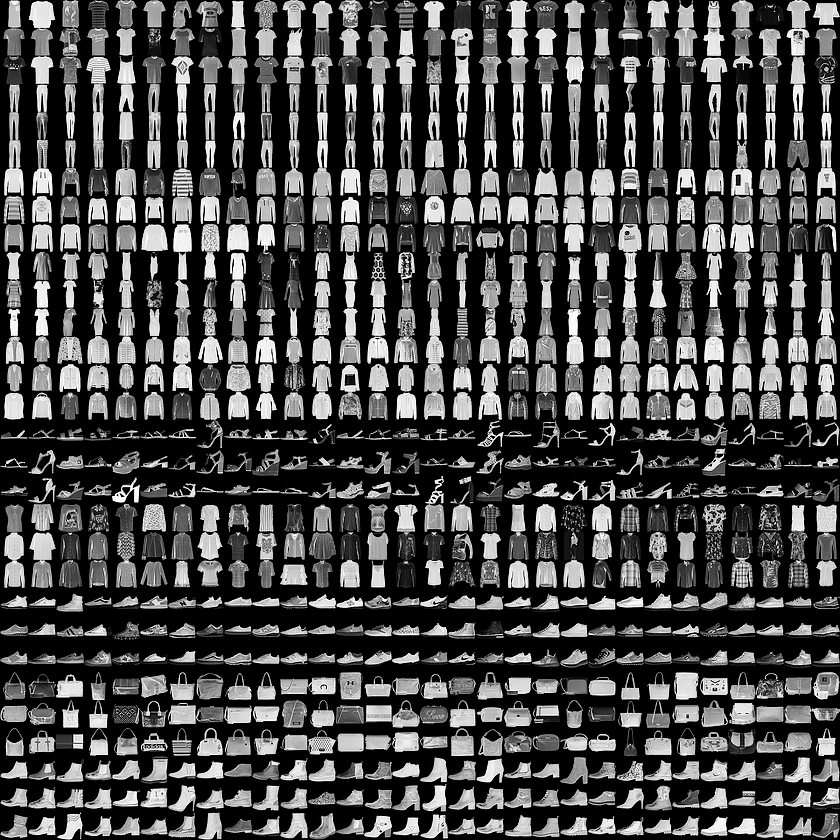
\includegraphics[width=\columnwidth]{images/fashion-mnist-sprite.png}
    \caption{Immagini estratte dal dataset Fashion-MNIST (tre righe per classe)}
    \label{fig1:fashion-MNIST}
\end{figure}
La nascita di Fashion-MNIST è dovuta al sovrautilizzo del noto dataset MNIST database of handwritten digit  \cite{lecun1998mnist}, utilizzato come punto di riferimento dalla comunità scientifica. Gli autori infatti spiegano che MNIST handrwitten è un dataset "troppo facile" dato che le reti convoluzionali riescono a raggiungere un punteggio del 99,7\% ed anche gli algoritmi classici di Machine Learning riesco a ottenere facilmente score del 97\%. L'esperto di deep learning François Chollet, creatore di Keras \cite{chollet2015keras}, ha dichiarato nell'Aprile del 2017 attraverso il proprio profilo \href{https://twitter.com/fchollet/status/852594987527045120}{Twitter} che MNIST non è rappresentativo dei moderni task di CV.\par
Per il task in questione sono state utilizzate due soluzioni architetturali differenti di reti neurali convoluzionali, le reti di questo tipo sono infatti disegnate per processare i dati disposti a griglia (come accade per i pixel di un'immagine). Una rete convoluzionale è un caso speciale di rete neurale che utilizza la convoluzione in almeno uno dei suoi layer. Le architetture proposte sono:
\begin{itemize}
\item CustomNet
\item ResNet-18 \cite{he2016deep}
\end{itemize}
CustomNet è un'architettura molto semplice progettata da zero ed è costituita da 3 layer convoluzionali e da un ultimo layer fully connected. ResNet-18 è invece il modello proposto da He \etal{} opportunamente riadattato per lo specifico compito in questione.\par
Infine sono state testate le soluzioni architetturali proposte valutandone le performance grazie alle metriche di accuracy, precision e recall.
